\chapter{Analiza systemowa i specyfikacja wymagań}

W niniejszym rozdziale przeprowadzono szczegółową analizę funkcjonalną systemu FasterPost, identyfikując kluczowych aktorów oraz definiując scenariusze ich interakcji z aplikacją. Celem tej analizy było stworzenie precyzyjnego modelu wymagań, który posłużył jako fundament dla późniejszego procesu projektowania architektury oraz implementacji poszczególnych modułów oprogramowania.

\section{Charakterystyka aktorów systemu}

Na podstawie analizy dziedziny problemu oraz wymagań biznesowych wyodrębniono trzy główne grupy użytkowników (aktorów), którzy wchodzą w bezpośrednią interakcję z systemem. Każda z ról posiada odrębny zakres odpowiedzialności oraz dedykowany interfejs użytkownika.

Pierwszym i najważniejszym aktorem jest \textbf{Klient}. Jest to użytkownik końcowy, będący inicjatorem procesu logistycznego. W ramach systemu FasterPost rola ta została podzielona na użytkowników niezarejestrowanych, którzy posiadają dostęp jedynie do podstawowych informacji ofertowych oraz śledzenia przesyłek, oraz użytkowników zarejestrowanych. Klient zalogowany dysponuje pełnym wachlarzem funkcjonalności, obejmującym nadawanie przesyłek, zarządzanie książką adresową, dokonywanie płatności online oraz przegląd historii zleceń. Interakcja Klienta z systemem odbywa się głównie poprzez responsywną aplikację internetową.

Drugą kluczową rolę pełni \textbf{Kurier}. Jest to pracownik terenowy, odpowiedzialny za fizyczną realizację transportu przesyłek w ramach tzw. "Ostatniej Mili" (Last Mile) oraz transportu międzyhubowego. Aktor ten korzysta ze specjalistycznego modułu aplikacji, dostosowanego do urządzeń mobilnych. Jego głównym zadaniem jest odbiór paczek z maszyn nadawczych, transport do magazynu oraz dystrybucja do paczkomatów docelowych. System wspiera Kuriera poprzez automatyczne wyznaczanie optymalnych tras przejazdu oraz weryfikację dostępności skrytek w czasie rzeczywistym.

Trzecim aktorem jest \textbf{Administrator}. Rola ta posiada najwyższy poziom uprawnień i odpowiada za utrzymanie ciągłości działania systemu. Administrator nie bierze bezpośredniego udziału w procesie przemieszczania paczek, lecz sprawuje nadzór techniczny i operacyjny. Do jego obowiązków należy zarządzanie kontami użytkowników, monitorowanie stanu technicznego infrastruktury (paczkomatów) oraz interwencja w przypadku wystąpienia błędów krytycznych lub reklamacji.

\section{Model przypadków użycia}

Diagram przypadków użycia (UML Use Case Diagram) stanowi wizualną reprezentację funkcjonalności systemu, obrazując relacje między zidentyfikowanymi aktorami a usługami oferowanymi przez aplikację FasterPost. Poniższy rysunek (Rys. \ref{fig:usecase}) przedstawia kompleksowy widok procesów biznesowych zaimplementowanych w projekcie.

\begin{figure}[htbp]
    \centering
    % Osadzenie pliku EPS.
    % Parametr width=1.0\textwidth dopasowuje szerokość do marginesów tekstu.
    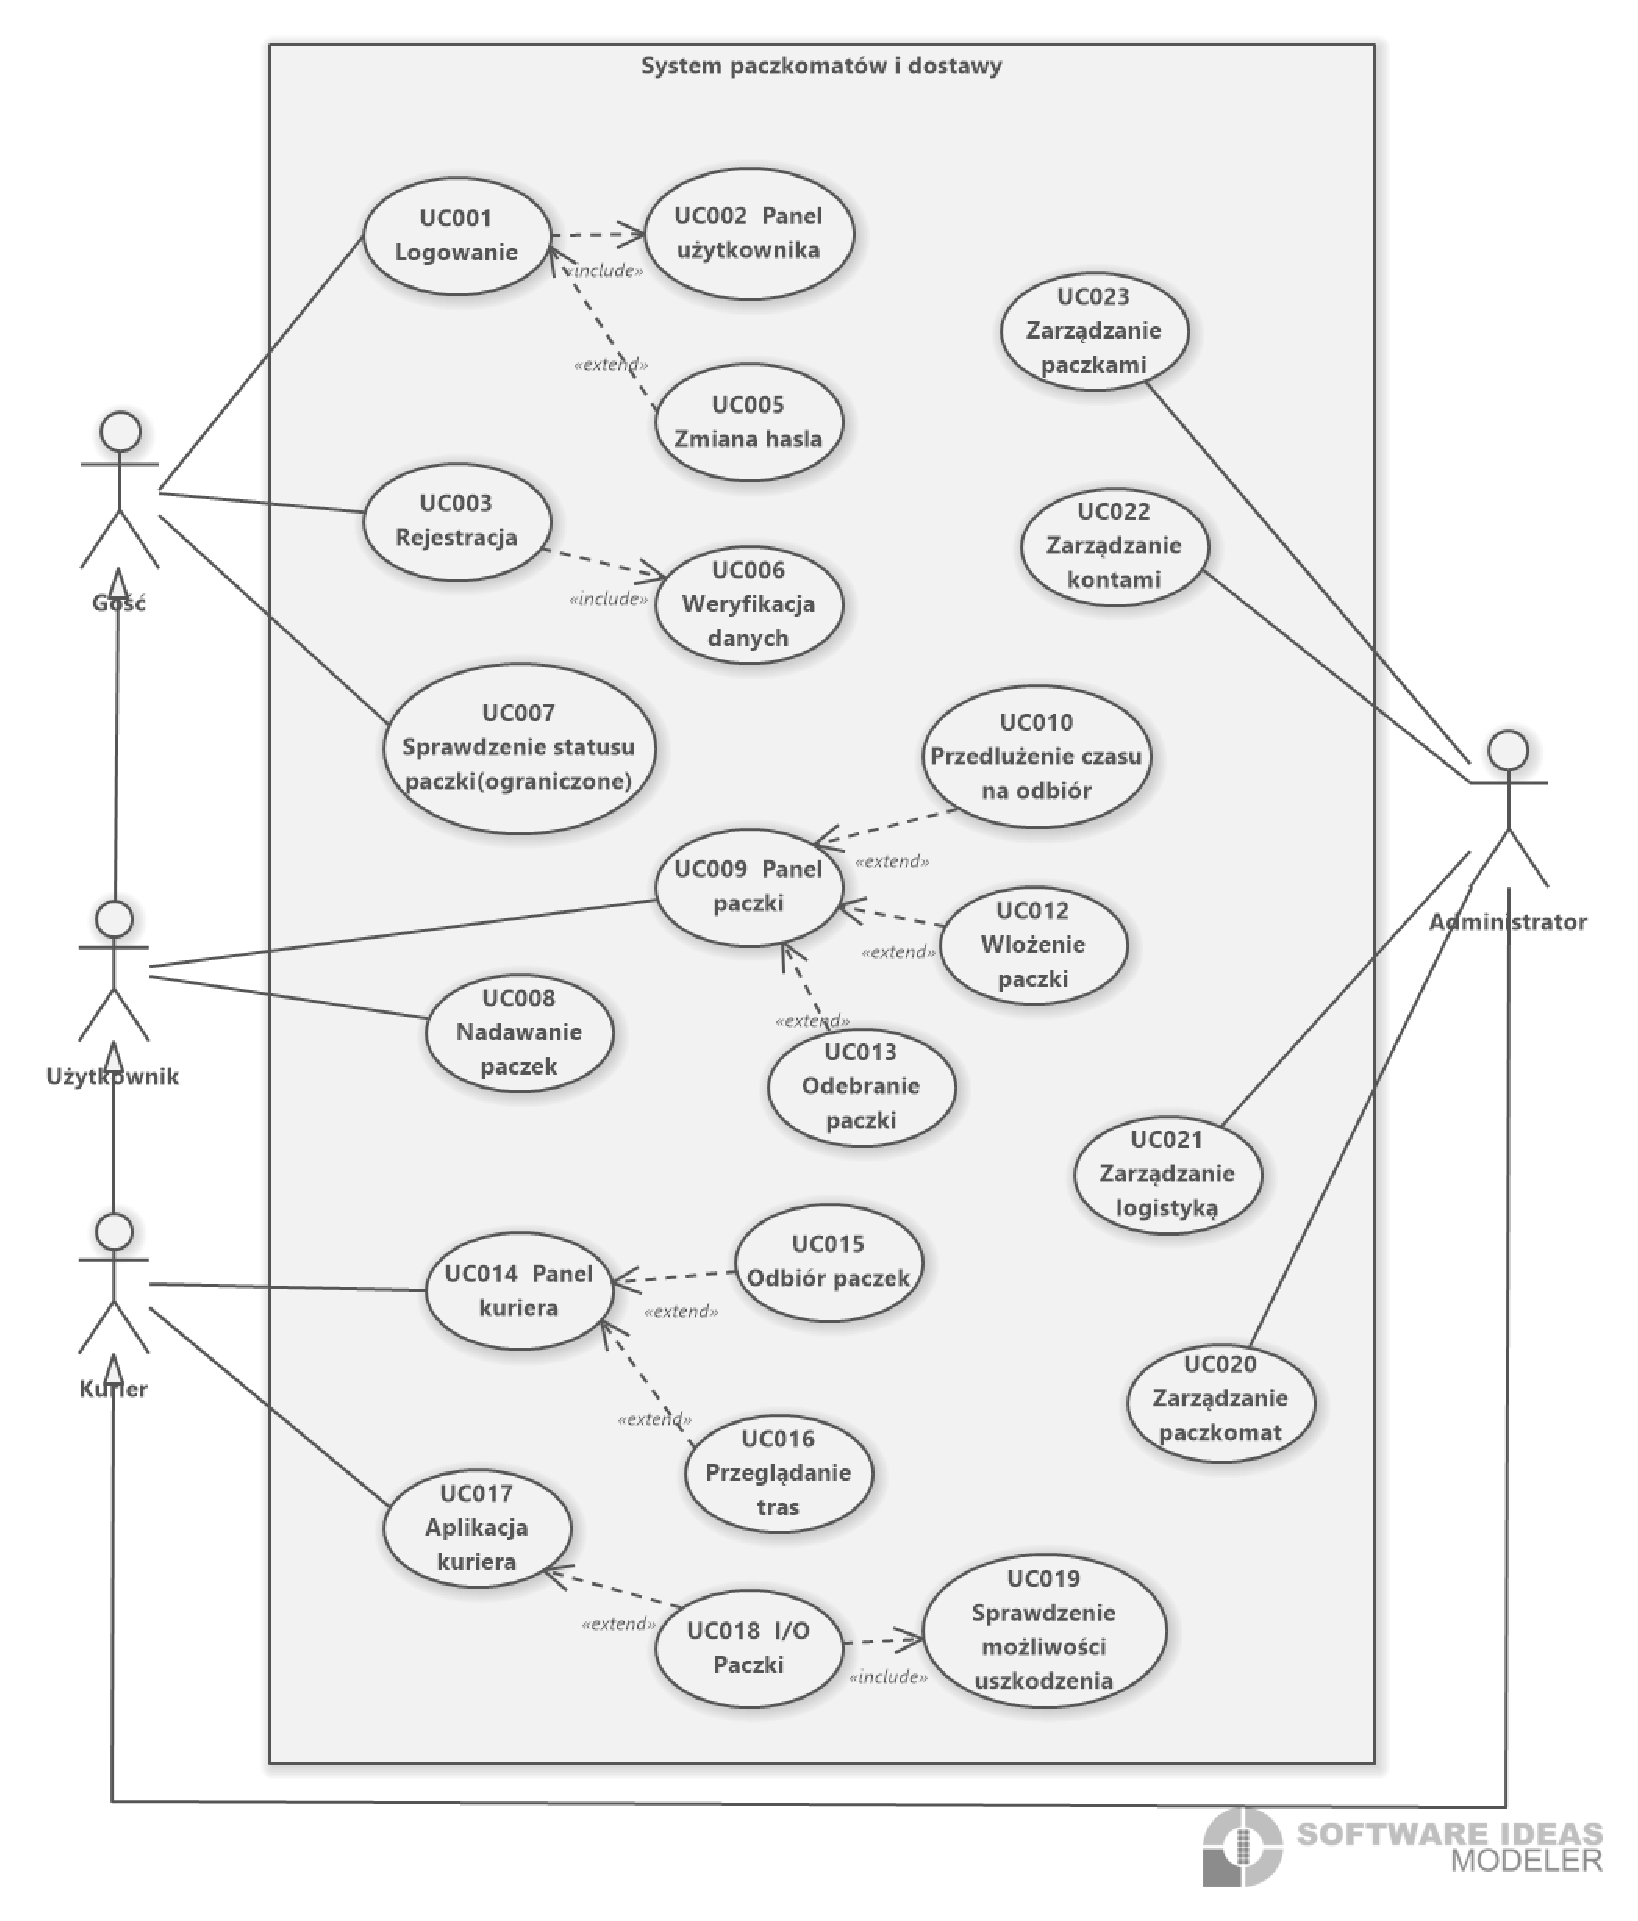
\includegraphics[width=1.0\textwidth]{figures/chapter2/UseCaseDiagram1.eps}
    \caption{Diagram przypadków użycia systemu FasterPost}
    \label{fig:usecase}
\end{figure}

Centralnym punktem diagramu jest system zarządzania przesyłkami, który integruje działania wszystkich aktorów. Wyraźnie widoczny jest podział na strefę klienta (inicjacja zlecenia) oraz strefę operacyjną (realizacja zlecenia przez kuriera i nadzór administratora).

\section{Szczegółowy opis scenariuszy biznesowych}

Poniżej przedstawiono narracyjny opis kluczowych procesów, które zostały zwizualizowane na diagramie przypadków użycia.

\subsection{Proces nadania przesyłki}

Proces nadania jest najbardziej złożonym scenariuszem po stronie Klienta. Rozpoczyna się on w momencie wyboru opcji "Nadaj paczkę" w panelu użytkownika. System wymaga od Klienta zdefiniowania parametrów fizycznych przesyłki (gabaryt S, M lub L) oraz wskazania danych adresata. Kluczowym elementem jest wybór punktów infrastrukturalnych – paczkomatu nadawczego oraz docelowego. System, wykorzystując dane geolokalizacyjne, sugeruje najbliższe dostępne maszyny.

Po zatwierdzeniu danych następuje proces płatności elektronicznej. System integruje się z zewnętrznym operatorem płatności, oczekując na potwierdzenie transakcji. Po pomyślnej autoryzacji płatności, system FasterPost automatycznie generuje etykietę przewozową oraz unikalny kod QR. Równocześnie następuje asynchroniczna komunikacja z wybranym paczkomatem nadawczym w celu wstępnej rezerwacji skrytki.

\subsection{Obsługa logistyczna i kurierska}

Z perspektywy Kuriera, praca z systemem rozpoczyna się od pobrania listy zadań (tzw. manifestu) na dany dzień. Aplikacja mobilna, komunikując się z API backendu, pobiera zoptymalizowaną trasę przejazdu, wyznaczoną algorytmami heurystycznymi. Kurier, docierając do paczkomatu, autoryzuje się w systemie maszyny, co umożliwia mu masowe otwarcie skrytek zawierających paczki do odbioru.

Każda operacja fizyczna na paczce (wyjęcie, załadunek na samochód, umieszczenie w magazynie) jest odnotowywana w systemie poprzez zeskanowanie kodu przesyłki. Dzięki temu status zamówienia jest aktualizowany w czasie rzeczywistym, co pozwala Klientowi na bieżące śledzenie losów przesyłki. W przypadku próby doręczenia paczki do przepełnionego paczkomatu, system dynamicznie weryfikuje dostępność skrytek i w razie potrzeby sugeruje Kurierowi alternatywne działania lub relokację przesyłki do magazynu buforowego.

\subsection{Zarządzanie i administracja}

Scenariusze administracyjne są niewidoczne dla zwykłego użytkownika, lecz kluczowe dla bezpieczeństwa danych. Administrator, logując się do dedykowanego panelu, ma możliwość przeglądu wszystkich transakcji i statusów w systemie. W sytuacjach awaryjnych, np. uszkodzenia drzwiczek w paczkomacie, Administrator ma możliwość zdalnego zablokowania konkretnej skrytki lub całej maszyny, wyłączając ją z puli dostępnych punktów dla nowych zleceń. Proces ten zapobiega frustracji użytkowników i zapewnia płynność działania sieci logistycznej.